\documentclass[tikz, border=2pt]{standalone}

\usepackage[dvipsnames]{xcolor}
\usetikzlibrary{arrows.meta, positioning}

\newcommand{\PredWR}{\mathsf{PredWR}}
\newcommand{\PredRW}{\mathsf{PredRW}}
\newcommand{\WW}{\mathsf{WW}}

\begin{document}
  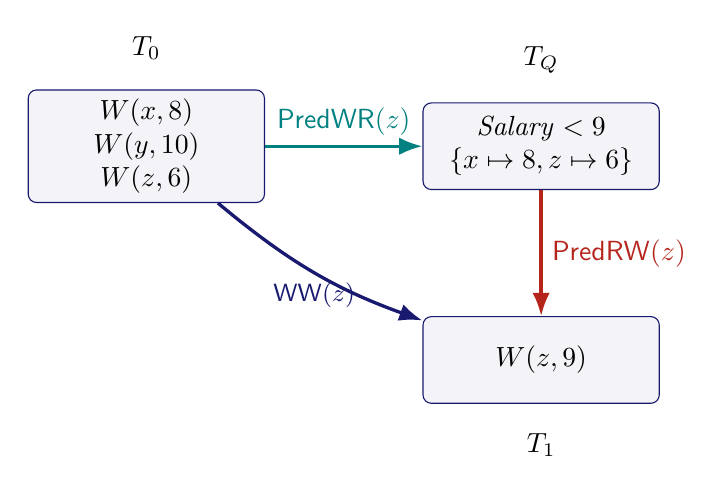
\begin{tikzpicture}[
      >=Latex,
      font = \normalsize,
      tx/.style={
        draw = MidnightBlue,
        rounded corners = 3pt,
        fill = MidnightBlue!5,
        minimum width = 30mm,
        minimum height = 11mm,
        align = center,
      },
    ]
    \node[tx] (w) {$W(x,8)$\\$W(y,10)$\\$W(z,6)$};
    \node[tx, right = 20mm of w] (q)
      {$\mathit{Salary}<9$\\$\{x\mapsto 8, z\mapsto 6\}$};
    \node[tx, below = 16mm of q] (u) {$W(z,9)$};
    \node[above = 2.5mm of w] {\textbf{$T_0$}};
    \node[above = 2.5mm of q] {\textbf{$T_Q$}};
    \node[below = 2.5mm of u] {\textbf{$T_1$}};
    \draw[-Latex, very thick, teal]
      (w) -- node[above] {$\PredWR(z)$} (q);
    \draw[-Latex, very thick, BrickRed]
      (q) -- node[right] {$\PredRW(z)$} (u);
    \draw[-Latex, very thick, MidnightBlue]
      (w) to[bend right = 10] node[below, font = \small] {$\WW(z)$} (u);
  \end{tikzpicture}
\end{document}
